\documentclass[../main.tex]{subfiles}

\begin{document}

\chapter{Alogrithms}

This appendix details the applied encryption and decryption algorithms.

\section{Encryption algorithm}
\label{app:encryption}
Figure \ref{app:encryption_algo} depicts the encryption algorithm in detail.
It takes a \textit{signed log} and a set of receivers as input and computes a JWE token which can only be decrypted by the defined users.
Internally, it computes and signs a \textit{shared header} and a \textit{shared log}.
Both are JWS-tokens.
The \textit{shared header} is passed as plaintext to the JWE encryption algorithm which is based on hybrid encryption.
First, a symmetric encryption scheme encrypts the \textit{shared header} under a symmetric key.
This key is then encrypted using asymmetric encryption algorithms.
The final JWE token consists of the encrypted \textit{shared header}, the encrypted keys and the \textit{shared header}.

\begin{figure}[h!]
    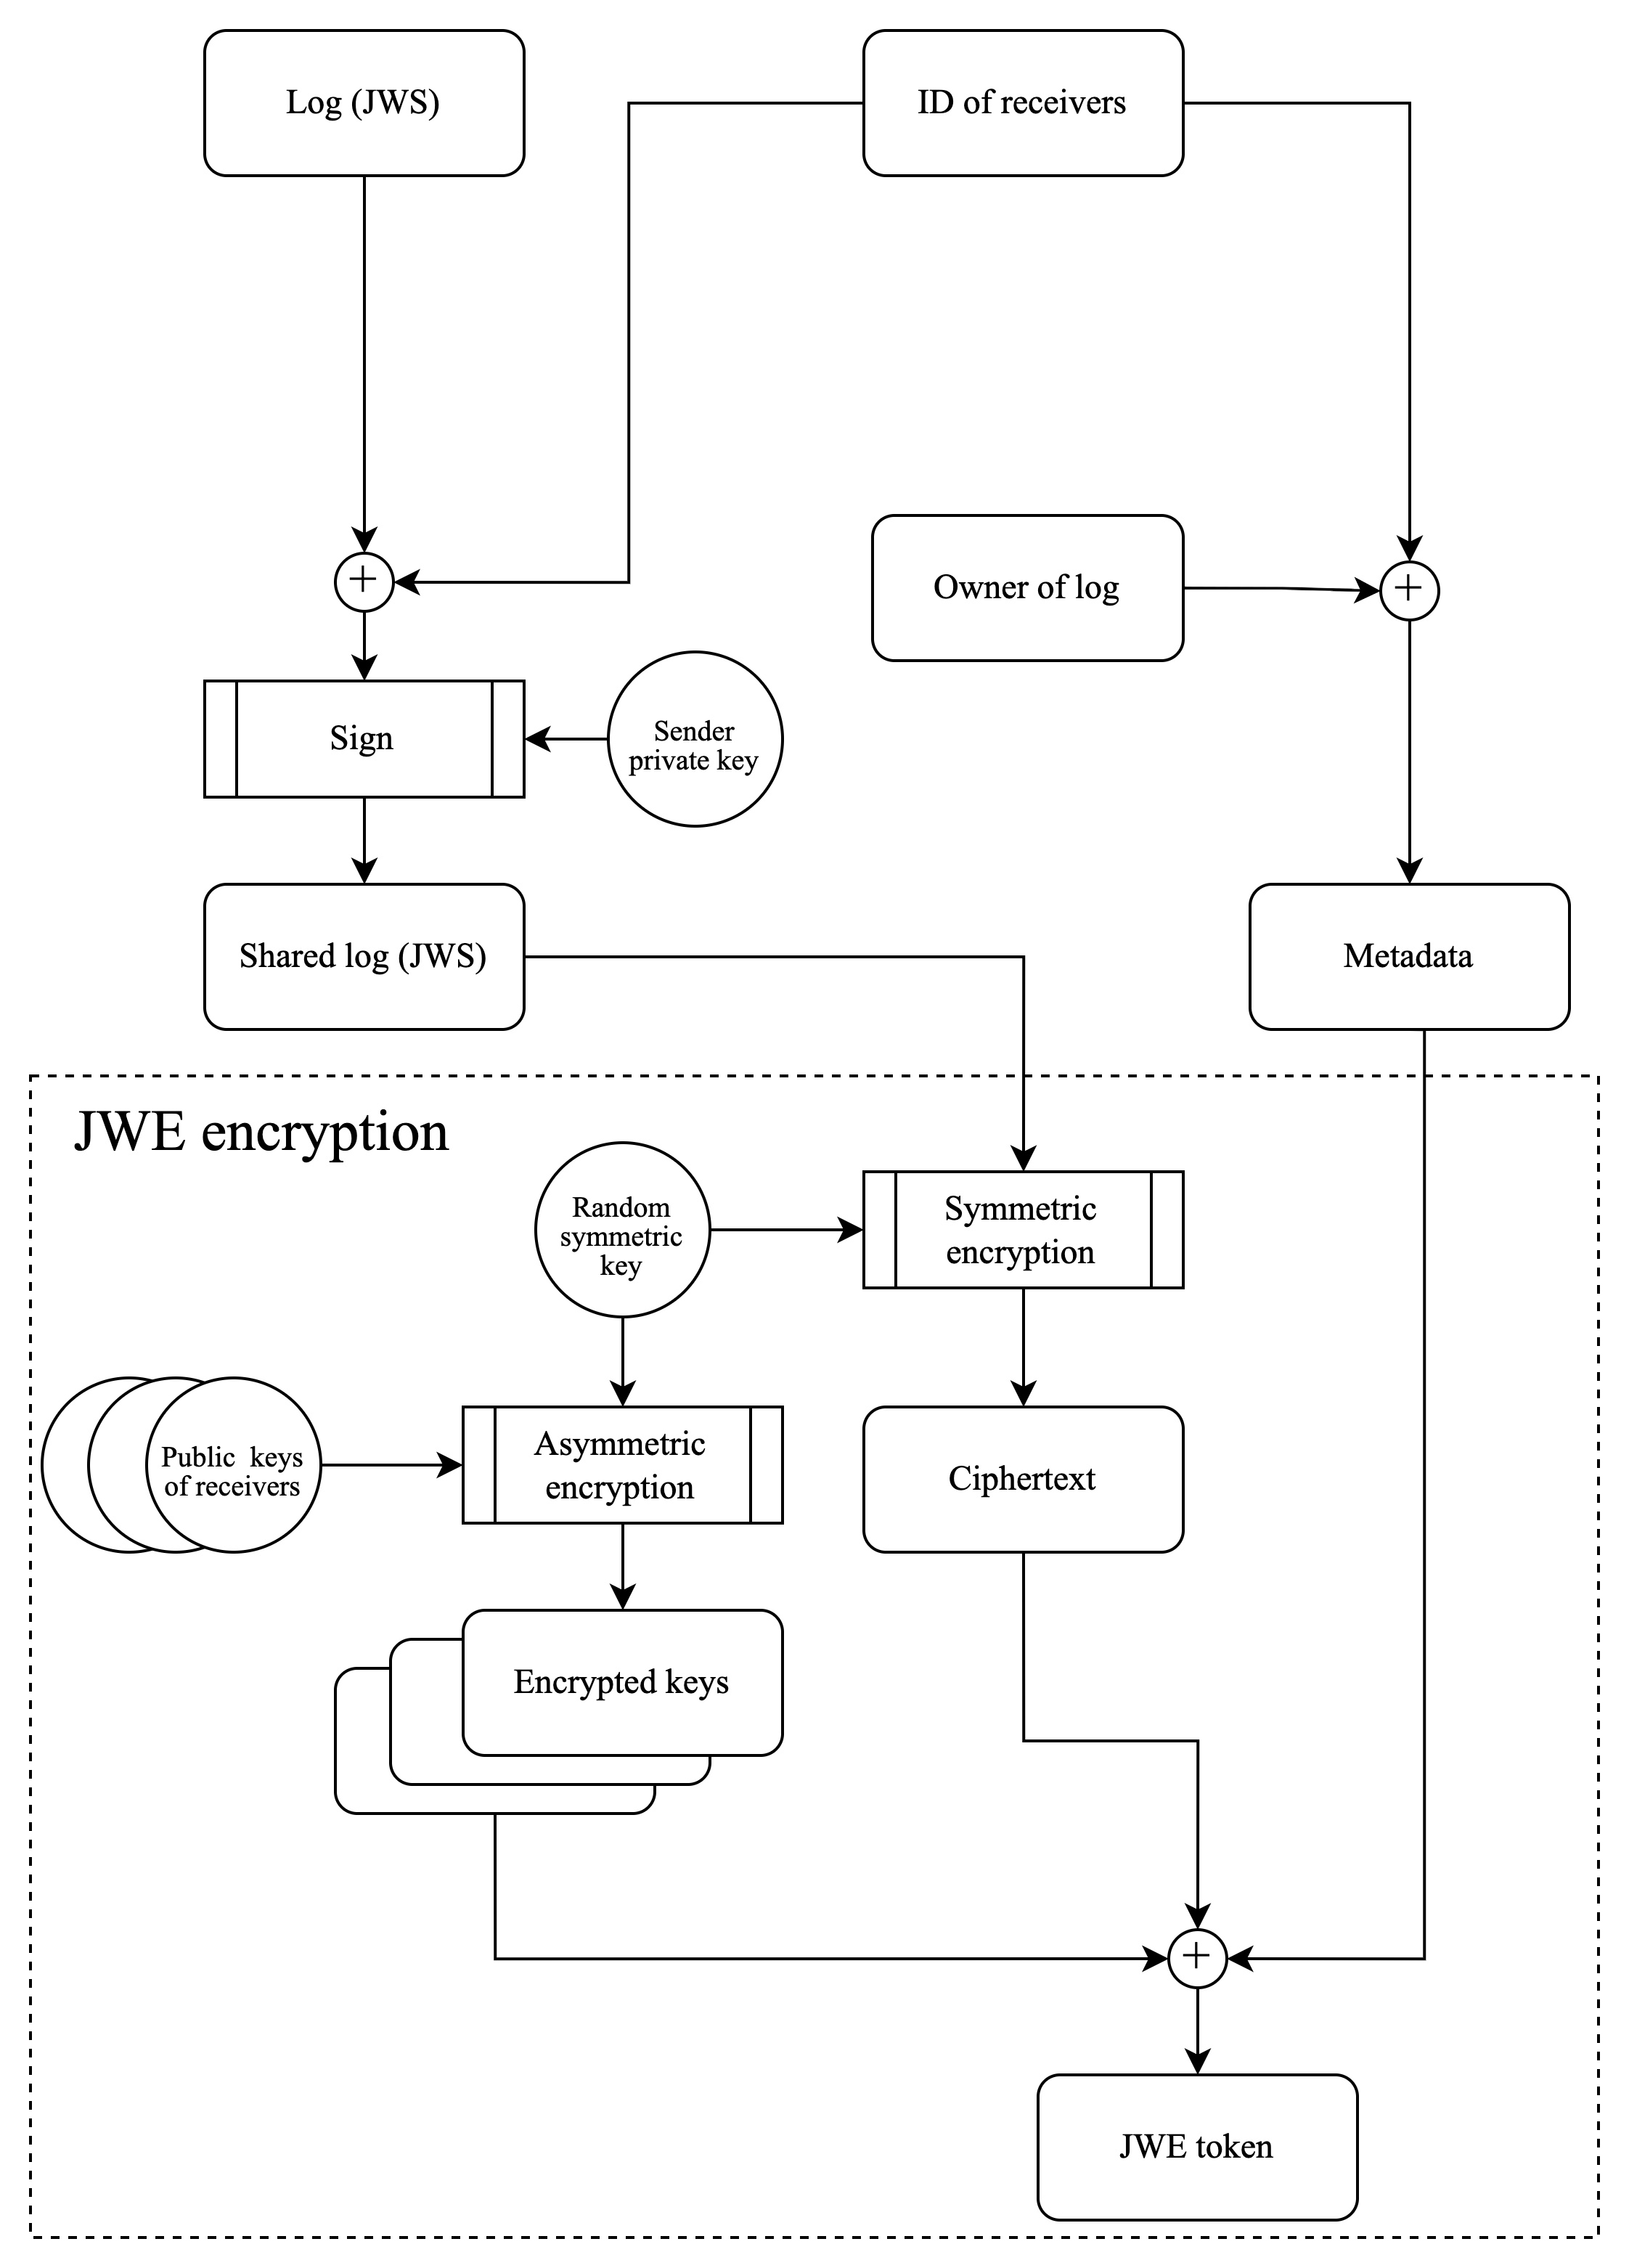
\includegraphics[scale=0.12]{../img/05/encrypt_logs.jpg}
    \centering
    \caption{The encryption algorithm takes a signed log and a set of receivers as input. It returns a JWE-token which can only be decrypted by the specified set of users.}
    \label{app:encryption_algo}
\end{figure}


\section{Decryption algorithm}
\label{app:decryption}
Figure \ref{app:encryption_algo} depicts the encryption algorithm in detail.
\begin{figure}[h]
    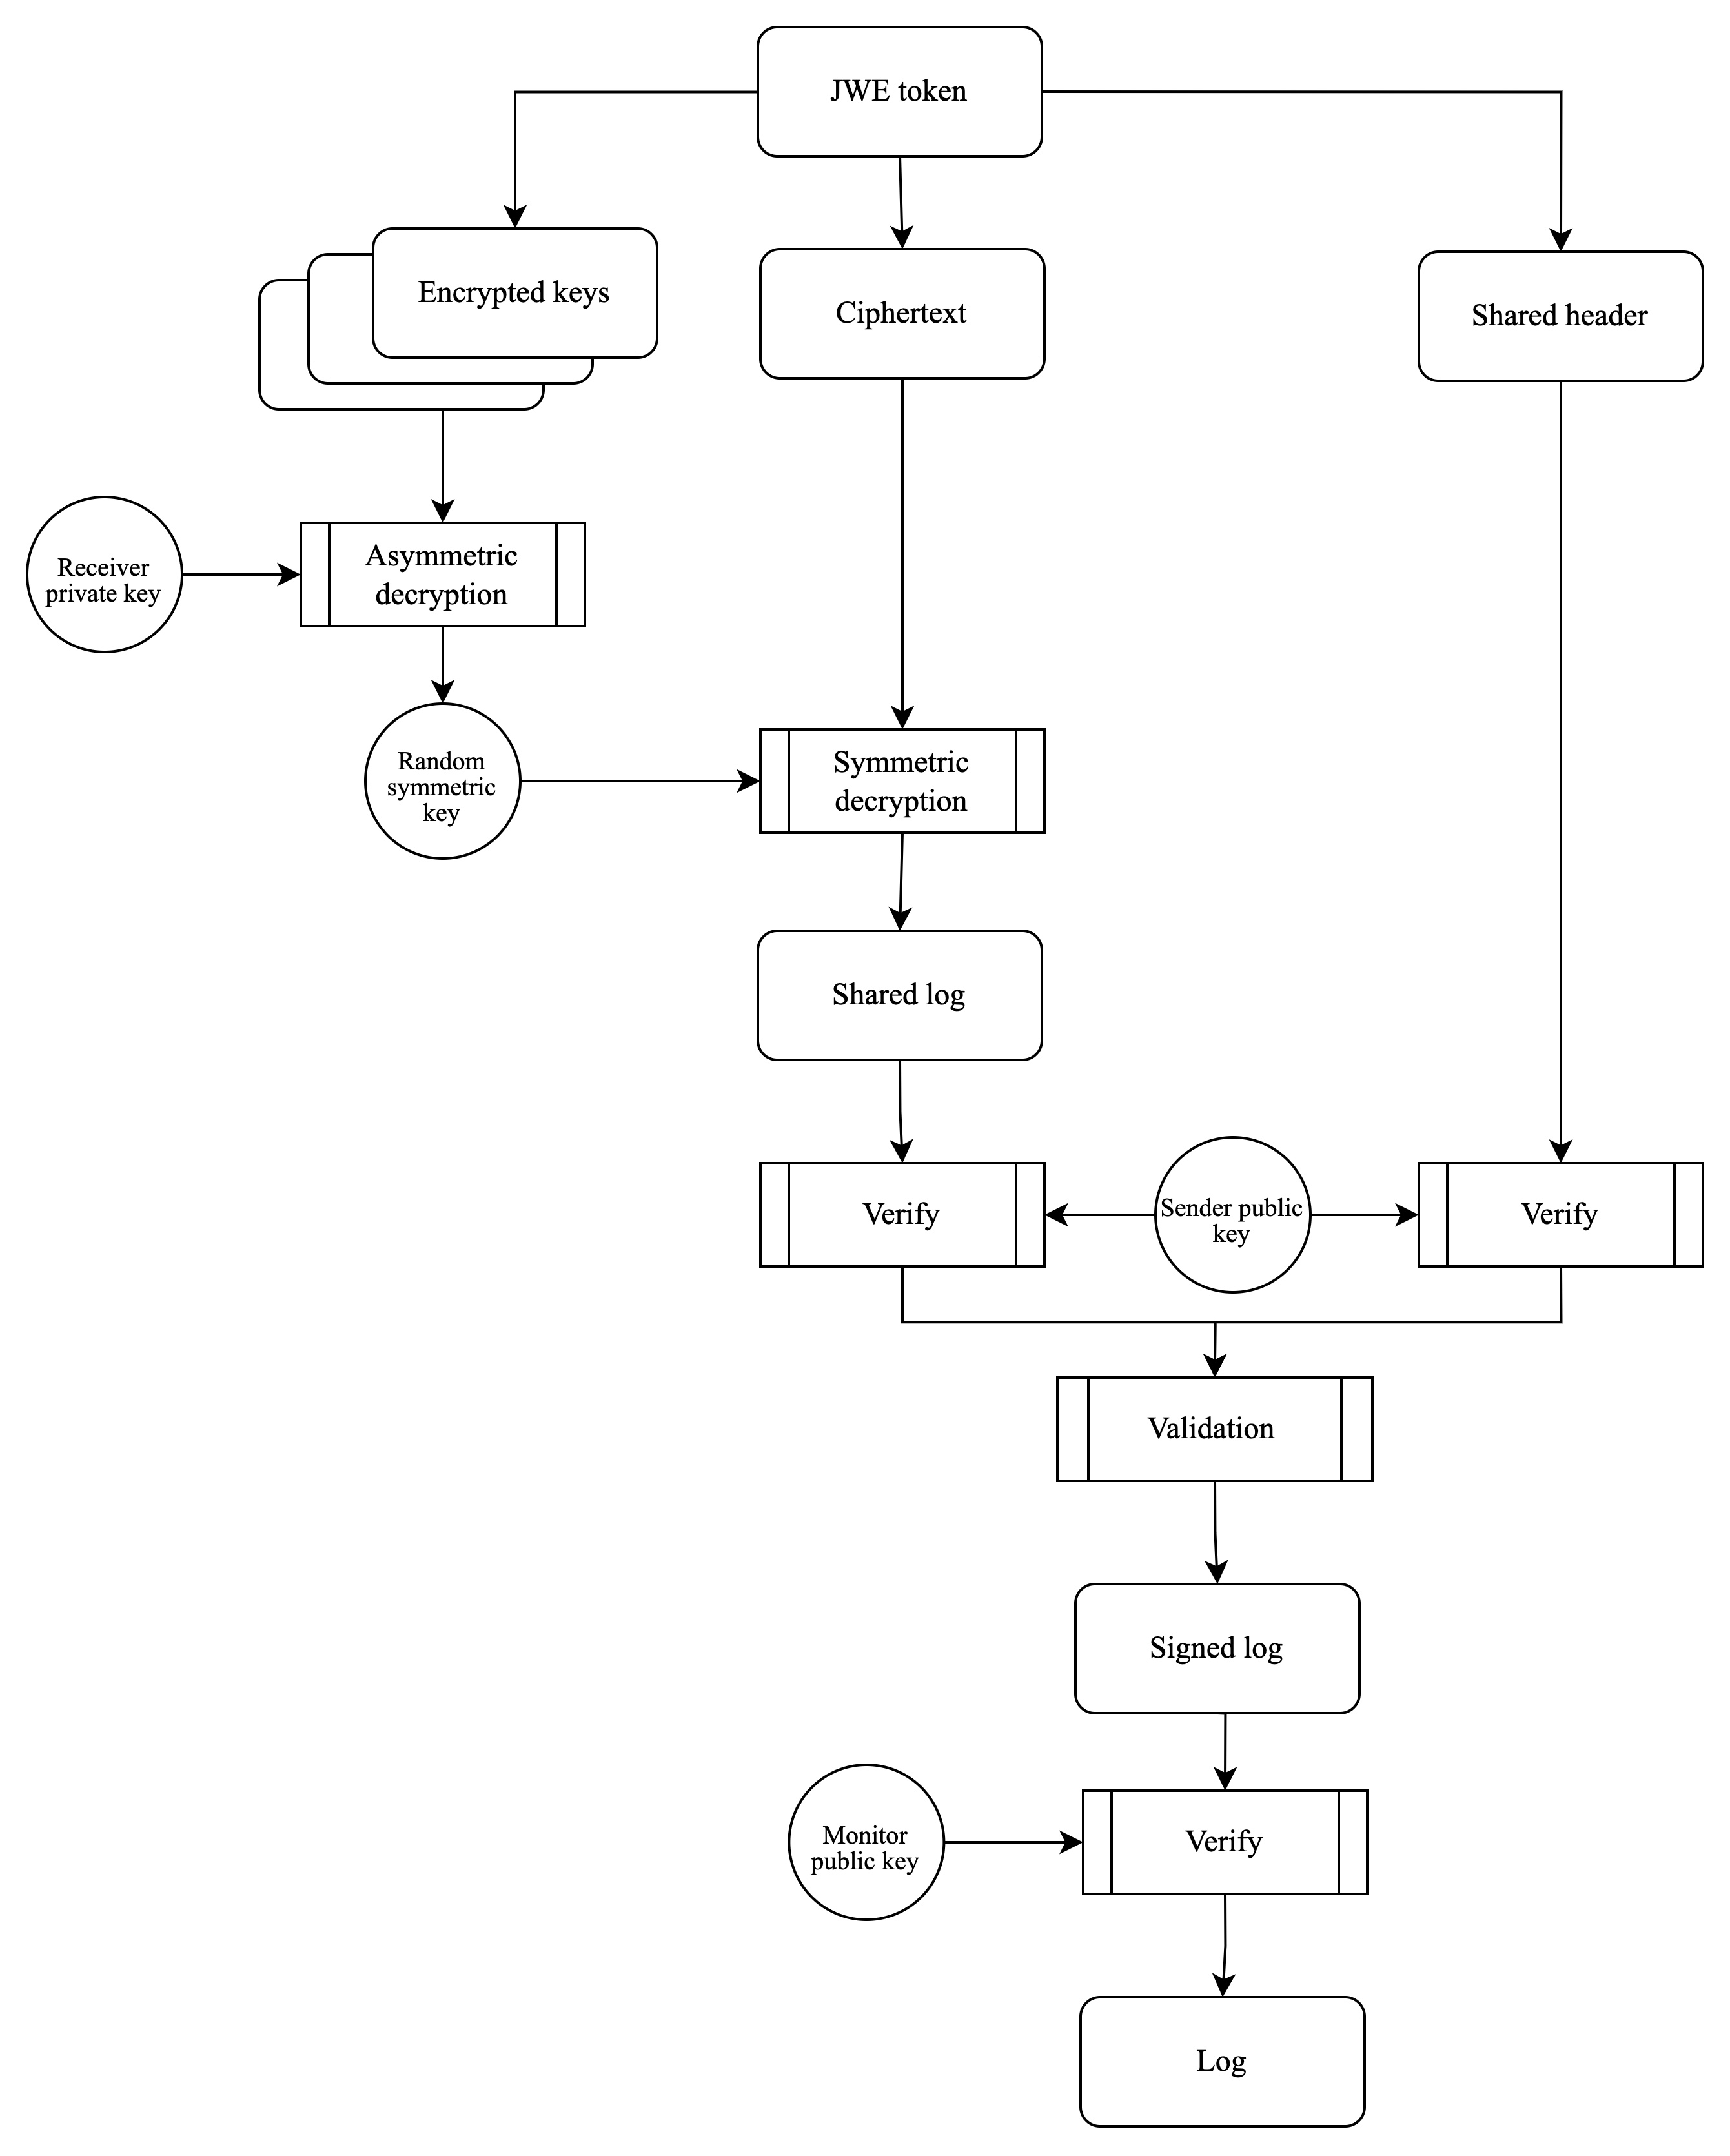
\includegraphics[scale=0.15]{../img/05/decrypt_logs.jpg}
    \centering
    \caption{The decryption algorithm takes a JWE token and a private decryption key as input. It returns the \textit{signed log} if the user .}
    \label{app:decryption_algo}
\end{figure}


\end{document}
